\chapter{Introduction}\label{ch:introduction}

% -------------------------------------------------------------------
\section{Problem Statement}\label{sec:introduction:problem_statement}
% -------------------------------------------------------------------

\glspl{amr} have gained enormous significance in the industrial sector over the last decade. They are used to improve operational efficiency, precision, and safety. In order to understand and navigate through the environment independently, the \glspl{amr} are required to run computation- and memory-intensive algorithms related to image processing, path planning, \gls{slam}, and learning \cite{Saeik2021}. However, this poses a challenge for the robot's onboard system, which has limited computational capabilities due to size and cost limitations as well as battery life \cite{Baxi2022}. Furthermore, these algorithms are time-sensitive and can cause operational failure for the \glspl{amr} if the latency restrictions cannot be satisfied. It becomes essential for large automated factories using \glspl{amr} to address this problem. 

\begin{figure}[htb]
    \centering

    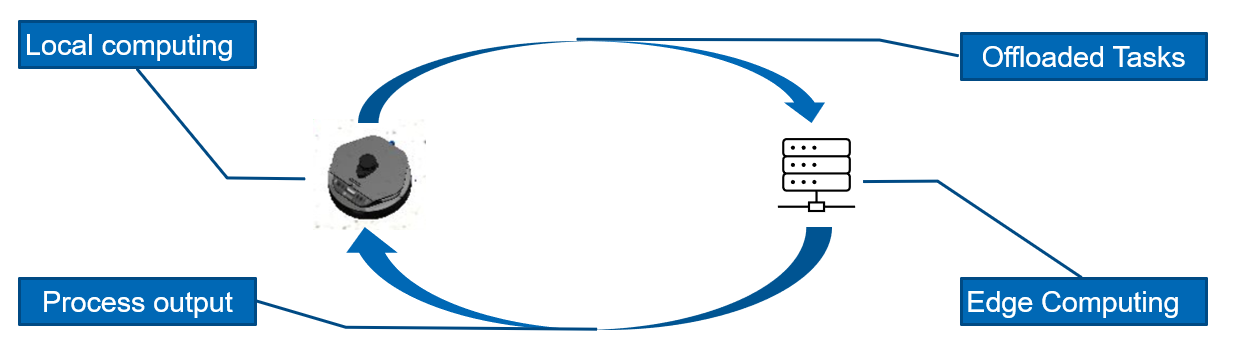
\includegraphics[width=0.8\linewidth]{figures/setup/amr_offloading.png}
    \caption[Computation offloading between \acrshort{amr} and edge computer]{This figure shows the computation offloading between the \gls{amr} and the edge computer. The \gls{amr} can choose to compute the tasks locally or to offload them to the edge computer. If the \gls{amr} chooses to offload, the edge computer will compute the tasks and send the processed output back to the \gls{amr} via the network} 

    \label{fig:amr_offloading}
\end{figure}

Edge computing as an evolution of cloud computing brings application hosting from data centers down to the edge of the network, where the data were initially collected, to achieve low latency and bandwidth efficiency \cite{Lin2019}. For latency-sensitive tasks on \glspl{amr}, such as perception and navigation, Edge computing offers an opportunity to enable the \glspl{amr} with limited resources by offloading costly computation tasks to the edge, while only a small portion of the computation remains on the \gls{amr}'s on-board system. An illustration of computation offloading between the \gls{amr} and the edge computer is shown in \cref{fig:amr_offloading}.

However, depending on the application scenarios, offloading certain tasks from \glspl{amr} to the edge at all times may not be possible, beneficial, or even feasible due to the network's latency, dynamic network changes, and resource availability. \citeauthor*{Baxi2022} \cite{Baxi2022} point out that a simple perception task using an RGB-D camera can cause over 100 ms sensing-to-actuation round-trip latency and over 400 Mbps network bandwidth usage. On the other hand, offloading computational workloads to the edge could also impact the \gls{amr}'s safety, availability as well as on-board resources. The exact influence on the robotic system will depend on the chosen offloading strategy. Therefore, it is necessary to investigate the effects of certain offloading strategies on the \gls{amr}'s safety, availability, and task performance.

% ---------------------------------------------------------------------
\section{Motivation}\label{sec:motivation}
% ---------------------------------------------------------------------

A number of works have investigated the computation offloading strategies as a purely mathematical problem and have proposed different algorithms to solve the problem. However, few of them consider the real application in \glspl{amr}, where the dynamic network changes and onboard resource limitations can affect the performance of the offloading strategies greatly. Therefore, the purpose of this thesis is to investigate the influence of different offloading strategies using actual robotic systems and edge computers in an experimental way.

 With the results from the experiments, this thesis is trying to answer the following research questions: What effects do different offloading strategies have on the specified metrics? Furthermore, this thesis is trying to answer the question: If and how the effects of different offloading strategies vary under different circumstances and if they have any (application-specific) constraints. Finally, this thesis is trying to gain insights if more complex strategies to achieve better results on the metrics. 

 Furthermore, this thesis aims to develop a dynamic offloading strategy that can detect the limitations of the available resources on different systems and can adapt to dynamic changes in network conditions, in order to minimize the execution latency of the offloaded computation task and improve its performance by using edge computers equipped with more computation resources.

% -------------------------------------------------------
\section{Research Methodology}\label{sec:research_methodology}
% -------------------------------------------------------

In order to carry out the experiments, an offloading framework for robot perception is implemented using \gls{ros}2 \cite{Macenski2022} and used to analyze the effects of different offloading strategies. More specifically, this thesis considers a 2D object detection task using the YOLOv5 models, proposed by \citeauthor*{Jocher2022} \cite{Jocher2022}. YOLOv5n, a smaller variant of the perception model, will be deployed on the \gls{amr}'s on-board system, while the edge counterpart uses a more accurate but also a more complex variant, e.g., YOLOv5l. The environment is an industrial warehouse containing different objects as obstacles, which is a common use case for \glspl{amr}. The \gls{amr} is equipped with camera sensors and uses navigation 2, proposed by \citeauthor*{Macenski2020} \cite{Macenski2020}, to navigate through a user-defined route.

First, the baseline strategies are investigated. More specifically, an "edge only" strategy that only offloads to the edge computer, a "robot only" strategy that only uses the \gls{amr}'s onboard system, and a series of strategies that offload to the edge with different ratios are used as the baseline strategies. This step aims to investigate the influence of different offloading strategies on the performance of the perception task and the resource usage of the \gls{amr} and the edge computer as well as the network. Then, a dynamic offloading strategy that makes decisions based on runtime parameters is developed and implemented, such as latency and \gls{amr}'s CPU usage and power consumption. This dynamic offloading strategy aims to minimize latency and improve the performance of the object detection task, inspired by the problem formulation of \citeauthor*{Ning2019} \cite{Ning2019}. Additional constraints subjected to power consumption and network bandwidth are applied to the algorithm. 

In the end, an evaluation framework is implemented based on important metrics of the object detection task performance and the \gls{amr}'s onboard resources. The baseline offloading strategies are first evaluated in simulation to verify the functionalities and the robustness of the offloading framework. Then, the experiments are carried out with an actual robotic system and evaluate the baseline strategies on the defined metrics. With results from the experiments with the baseline strategies, the dynamic offloading strategy is developed and evaluated against the baseline strategies by conducting experiments using Ethernet and Wi-Fi connections. 
